%%
%%

\addcontentsline{lof}{figure}{Smart Memory Allocation with Orphaned Buffer
Detection}
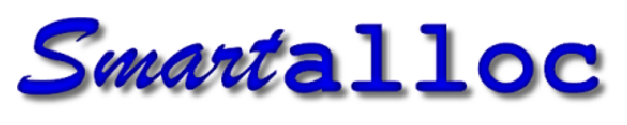
\includegraphics{./smartall.eps} 

\section*{Smart Memory Allocation With Orphaned Buffer Detection }
\label{_ChapterStart4}
\index{Detection!Smart Memory Allocation With Orphaned Buffer }
\index{Smart Memory Allocation With Orphaned Buffer Detection }
\addcontentsline{toc}{section}{Smart Memory Allocation With Orphaned Buffer
Detection}


Few things are as embarrassing as a program that leaks, yet few errors are so
easy to commit or as difficult to track down in a large, complicated program
as failure to release allocated memory. SMARTALLOC replaces the standard C
library memory allocation functions with versions which keep track of buffer
allocations and releases and report all orphaned buffers at the end of program
execution. By including this package in your program during development and
testing, you can identify code that loses buffers right when it's added and
most easily fixed, rather than as part of a crisis debugging push when the
problem is identified much later in the testing cycle (or even worse, when the
code is in the hands of a customer). When program testing is complete, simply
recompiling with different flags removes SMARTALLOC from your program,
permitting it to run without speed or storage penalties. 

In addition to detecting orphaned buffers, SMARTALLOC also helps to find other
common problems in management of dynamic storage including storing before the
start or beyond the end of an allocated buffer, referencing data through a
pointer to a previously released buffer, attempting to release a buffer twice
or releasing storage not obtained from the allocator, and assuming the initial
contents of storage allocated by functions that do not guarantee a known
value. SMARTALLOC's checking does not usually add a large amount of overhead
to a program (except for programs which use {\tt realloc()} extensively; see
below). SMARTALLOC focuses on proper storage management rather than internal
consistency of the heap as checked by the malloc\_debug facility available on
some systems. SMARTALLOC does not conflict with malloc\_debug and both may be
used together, if you wish. SMARTALLOC makes no assumptions regarding the
internal structure of the heap and thus should be compatible with any C
language implementation of the standard memory allocation functions. 

\subsubsection*{ Installing SMARTALLOC}
\index{SMARTALLOC!Installing }
\index{Installing SMARTALLOC }
\addcontentsline{toc}{subsubsection}{Installing SMARTALLOC}

SMARTALLOC is provided as a Zipped archive, 
\elink{smartall.zip}{http://www.fourmilab.ch/smartall/smartall.zip}; see the
download instructions below. 

To install SMARTALLOC in your program, simply add the statement: 

to every C program file which calls any of the memory allocation functions
({\tt malloc}, {\tt calloc}, {\tt free}, etc.). SMARTALLOC must be used for
all memory allocation with a program, so include file for your entire program,
if you have such a thing. Next, define the symbol SMARTALLOC in the
compilation before the inclusion of smartall.h. I usually do this by having my
Makefile add the ``{\tt -DSMARTALLOC}'' option to the C compiler for
non-production builds. You can define the symbol manually, if you prefer, by
adding the statement: 

{\tt \#define SMARTALLOC} 

At the point where your program is all done and ready to relinquish control to
the operating system, add the call: 

{\tt \ \ \ \ \ \ \ \ sm\_dump(}{\it datadump}{\tt );} 

where {\it datadump} specifies whether the contents of orphaned buffers are to
be dumped in addition printing to their size and place of allocation. The data
are dumped only if {\it datadump} is nonzero, so most programs will normally
use ``{\tt sm\_dump(0);}''. If a mysterious orphaned buffer appears that can't
be identified from the information this prints about it, replace the statement
with ``{\tt sm\_dump(1)};''. Usually the dump of the buffer's data will
furnish the additional clues you need to excavate and extirpate the elusive
error that left the buffer allocated. 

Finally, add the files ``smartall.h'' and ``smartall.c'' from this release to
your source directory, make dependencies, and linker input. You needn't make
inclusion of smartall.c in your link optional; if compiled with SMARTALLOC not
defined it generates no code, so you may always include it knowing it will
waste no storage in production builds. Now when you run your program, if it
leaves any buffers around when it's done, each will be reported by {\tt
sm\_dump()} on stderr as follows: 

\footnotesize
\begin{verbatim}
Orphaned buffer:     120 bytes allocated at line 50 of gutshot.c
\end{verbatim}
\normalsize

\subsubsection*{ Squelching a SMARTALLOC}
\index{SMARTALLOC!Squelching a }
\index{Squelching a SMARTALLOC }
\addcontentsline{toc}{subsubsection}{Squelching a SMARTALLOC}

Usually, when you first install SMARTALLOC in an existing program you'll find
it nattering about lots of orphaned buffers. Some of these turn out to be
legitimate errors, but some are storage allocated during program
initialisation that, while dynamically allocated, is logically static storage
not intended to be released. Of course, you can get rid of the complaints
about these buffers by adding code to release them, but by doing so you're
adding unnecessary complexity and code size to your program just to silence
the nattering of a SMARTALLOC, so an escape hatch is provided to eliminate the
need to release these buffers. 

Normally all storage allocated with the functions {\tt malloc()}, {\tt
calloc()}, and {\tt realloc()} is monitored by SMARTALLOC. If you make the
function call: 

\footnotesize
\begin{verbatim}
        sm_static(1);
\end{verbatim}
\normalsize

you declare that subsequent storage allocated by {\tt malloc()}, {\tt
calloc()}, and {\tt realloc()} should not be considered orphaned if found to
be allocated when {\tt sm\_dump()} is called. I use a call on ``{\tt
sm\_static(1);}'' before I allocate things like program configuration tables
so I don't have to add code to release them at end of program time. After
allocating unmonitored data this way, be sure to add a call to: 

\footnotesize
\begin{verbatim}
        sm_static(0);
\end{verbatim}
\normalsize

to resume normal monitoring of buffer allocations. Buffers allocated while
{\tt sm\_static(1}) is in effect are not checked for having been orphaned but
all the other safeguards provided by SMARTALLOC remain in effect. You may
release such buffers, if you like; but you don't have to. 

\subsubsection*{ Living with Libraries}
\index{Libraries!Living with }
\index{Living with Libraries }
\addcontentsline{toc}{subsubsection}{Living with Libraries}

Some library functions for which source code is unavailable may gratuitously
allocate and return buffers that contain their results, or require you to pass
them buffers which they subsequently release. If you have source code for the
library, by far the best approach is to simply install SMARTALLOC in it,
particularly since this kind of ill-structured dynamic storage management is
the source of so many storage leaks. Without source code, however, there's no
option but to provide a way to bypass SMARTALLOC for the buffers the library
allocates and/or releases with the standard system functions. 

For each function {\it xxx} redefined by SMARTALLOC, a corresponding routine
named ``{\tt actually}{\it xxx}'' is furnished which provides direct access to
the underlying system function, as follows: 

\begin{quote}

\begin{longtable}{ll}
\multicolumn{1}{l }{\bf Standard function } & \multicolumn{1}{l }{\bf Direct
access function  } \\
{{\tt malloc(}{\it size}{\tt )}  } & {{\tt actuallymalloc(}{\it size}{\tt )} 
} \\
{{\tt calloc(}{\it nelem}{\tt ,} {\it elsize}{\tt )}  } & {{\tt
actuallycalloc(}{\it nelem}, {\it elsize}{\tt )}   } \\
{{\tt realloc(}{\it ptr}{\tt ,} {\it size}{\tt )} } & {{\tt
actuallyrealloc(}{\it ptr}, {\it size}{\tt )}  } \\
{{\tt free(}{\it ptr}{\tt )} } & {{\tt actuallyfree(}{\it ptr}{\tt )} }

\end{longtable}

\end{quote}

For example, suppose there exists a system library function named ``{\tt
getimage()}'' which reads a raster image file and returns the address of a
buffer containing it. Since the library routine allocates the image directly
with {\tt malloc()}, you can't use SMARTALLOC's {\tt free()}, as that call
expects information placed in the buffer by SMARTALLOC's special version of
{\tt malloc()}, and hence would report an error. To release the buffer you
should call {\tt actuallyfree()}, as in this code fragment: 

\footnotesize
\begin{verbatim}
        struct image *ibuf = getimage("ratpack.img");
        display_on_screen(ibuf);
        actuallyfree(ibuf);
\end{verbatim}
\normalsize

Conversely, suppose we are to call a library function, ``{\tt putimage()}'',
which writes an image buffer into a file and then releases the buffer with
{\tt free()}. Since the system {\tt free()} is being called, we can't pass a
buffer allocated by SMARTALLOC's allocation routines, as it contains special
information that the system {\tt free()} doesn't expect to be there. The
following code uses {\tt actuallymalloc()} to obtain the buffer passed to such
a routine. 

\footnotesize
\begin{verbatim}
        struct image *obuf =
           (struct image *) actuallymalloc(sizeof(struct image));
        dump_screen_to_image(obuf);
        putimage("scrdump.img", obuf);  /* putimage() releases obuf */
\end{verbatim}
\normalsize

It's unlikely you'll need any of the ``actually'' calls except under very odd
circumstances (in four products and three years, I've only needed them once),
but they're there for the rare occasions that demand them. Don't use them to
subvert the error checking of SMARTALLOC; if you want to disable orphaned
buffer detection, use the {\tt sm\_static(1)} mechanism described above. That
way you don't forfeit all the other advantages of SMARTALLOC as you do when
using {\tt actuallymalloc()} and {\tt actuallyfree()}. 

\subsubsection*{ SMARTALLOC Details}
\index{SMARTALLOC Details }
\index{Details!SMARTALLOC }
\addcontentsline{toc}{subsubsection}{SMARTALLOC Details}

When you include ``smartall.h'' and define SMARTALLOC, the following standard
system library functions are redefined with the \#define mechanism to call
corresponding functions within smartall.c instead. (For details of the
redefinitions, please refer to smartall.h.) 

\footnotesize
\begin{verbatim}
        void *malloc(size_t size)
        void *calloc(size_t nelem, size_t elsize)
        void *realloc(void *ptr, size_t size)
        void free(void *ptr)
        void cfree(void *ptr)
\end{verbatim}
\normalsize

{\tt cfree()} is a historical artifact identical to {\tt free()}. 

In addition to allocating storage in the same way as the standard library
functions, the SMARTALLOC versions expand the buffers they allocate to include
information that identifies where each buffer was allocated and to chain all
allocated buffers together. When a buffer is released, it is removed from the
allocated buffer chain. A call on {\tt sm\_dump()} is able, by scanning the
chain of allocated buffers, to find all orphaned buffers. Buffers allocated
while {\tt sm\_static(1)} is in effect are specially flagged so that, despite
appearing on the allocated buffer chain, {\tt sm\_dump()} will not deem them
orphans. 

When a buffer is allocated by {\tt malloc()} or expanded with {\tt realloc()},
all bytes of newly allocated storage are set to the hexadecimal value 0x55
(alternating one and zero bits). Note that for {\tt realloc()} this applies
only to the bytes added at the end of buffer; the original contents of the
buffer are not modified. Initializing allocated storage to a distinctive
nonzero pattern is intended to catch code that erroneously assumes newly
allocated buffers are cleared to zero; in fact their contents are random. The
{\tt calloc()} function, defined as returning a buffer cleared to zero,
continues to zero its buffers under SMARTALLOC. 

Buffers obtained with the SMARTALLOC functions contain a special sentinel byte
at the end of the user data area. This byte is set to a special key value
based upon the buffer's memory address. When the buffer is released, the key
is tested and if it has been overwritten an assertion in the {\tt free}
function will fail. This catches incorrect program code that stores beyond the
storage allocated for the buffer. At {\tt free()} time the queue links are
also validated and an assertion failure will occur if the program has
destroyed them by storing before the start of the allocated storage. 

In addition, when a buffer is released with {\tt free()}, its contents are
immediately destroyed by overwriting them with the hexadecimal pattern 0xAA
(alternating bits, the one's complement of the initial value pattern). This
will usually trip up code that keeps a pointer to a buffer that's been freed
and later attempts to reference data within the released buffer. Incredibly,
this is {\it legal} in the standard Unix memory allocation package, which
permits programs to free() buffers, then raise them from the grave with {\tt
realloc()}. Such program ``logic'' should be fixed, not accommodated, and
SMARTALLOC brooks no such Lazarus buffer`` nonsense. 

Some C libraries allow a zero size argument in calls to {\tt malloc()}. Since
this is far more likely to indicate a program error than a defensible
programming stratagem, SMARTALLOC disallows it with an assertion. 

When the standard library {\tt realloc()} function is called to expand a
buffer, it attempts to expand the buffer in place if possible, moving it only
if necessary. Because SMARTALLOC must place its own private storage in the
buffer and also to aid in error detection, its version of {\tt realloc()}
always moves and copies the buffer except in the trivial case where the size
of the buffer is not being changed. By forcing the buffer to move on every
call and destroying the contents of the old buffer when it is released,
SMARTALLOC traps programs which keep pointers into a buffer across a call on
{\tt realloc()} which may move it. This strategy may prove very costly to
programs which make extensive use of {\tt realloc()}. If this proves to be a
problem, such programs may wish to use {\tt actuallymalloc()}, {\tt
actuallyrealloc()}, and {\tt actuallyfree()} for such frequently-adjusted
buffers, trading error detection for performance. Although not specified in
the System V Interface Definition, many C library implementations of {\tt
realloc()} permit an old buffer argument of NULL, causing {\tt realloc()} to
allocate a new buffer. The SMARTALLOC version permits this. 

\subsubsection*{ When SMARTALLOC is Disabled}
\index{When SMARTALLOC is Disabled }
\index{Disabled!When SMARTALLOC is }
\addcontentsline{toc}{subsubsection}{When SMARTALLOC is Disabled}

When SMARTALLOC is disabled by compiling a program with the symbol SMARTALLOC
not defined, calls on the functions otherwise redefined by SMARTALLOC go
directly to the system functions. In addition, compile-time definitions
translate calls on the ''{\tt actually}...{\tt ()}`` functions into the
corresponding library calls; ''{\tt actuallymalloc(100)}``, for example,
compiles into ''{\tt malloc(100)}``. The two special SMARTALLOC functions,
{\tt sm\_dump()} and {\tt sm\_static()}, are defined to generate no code
(hence the null statement). Finally, if SMARTALLOC is not defined, compilation
of the file smartall.c generates no code or data at all, effectively removing
it from the program even if named in the link instructions. 

Thus, except for unusual circumstances, a program that works with SMARTALLOC
defined for testing should require no changes when built without it for
production release. 

\subsubsection*{ The {\tt alloc()} Function}
\index{Function!alloc }
\index{Alloc() Function }
\addcontentsline{toc}{subsubsection}{alloc() Function}

Many programs I've worked on use very few direct calls to {\tt malloc()},
using the identically declared {\tt alloc()} function instead. Alloc detects
out-of-memory conditions and aborts, removing the need for error checking on
every call of {\tt malloc()} (and the temptation to skip checking for
out-of-memory). 

As a convenience, SMARTALLOC supplies a compatible version of {\tt alloc()} in
the file alloc.c, with its definition in the file alloc.h. This version of
{\tt alloc()} is sensitive to the definition of SMARTALLOC and cooperates with
SMARTALLOC's orphaned buffer detection. In addition, when SMARTALLOC is
defined and {\tt alloc()} detects an out of memory condition, it takes
advantage of the SMARTALLOC diagnostic information to identify the file and
line number of the call on {\tt alloc()} that failed. 

\subsubsection*{ Overlays and Underhandedness}
\index{Underhandedness!Overlays and }
\index{Overlays and Underhandedness }
\addcontentsline{toc}{subsubsection}{Overlays and Underhandedness}

String constants in the C language are considered to be static arrays of
characters accessed through a pointer constant. The arrays are potentially
writable even though their pointer is a constant. SMARTALLOC uses the
compile-time definition {\tt ./smartall.wml} to obtain the name of the file in
which a call on buffer allocation was performed. Rather than reserve space in
a buffer to save this information, SMARTALLOC simply stores the pointer to the
compiled-in text of the file name. This works fine as long as the program does
not overlay its data among modules. If data are overlayed, the area of memory
which contained the file name at the time it was saved in the buffer may
contain something else entirely when {\tt sm\_dump()} gets around to using the
pointer to edit the file name which allocated the buffer. 

If you want to use SMARTALLOC in a program with overlayed data, you'll have to
modify smartall.c to either copy the file name to a fixed-length field added
to the {\tt abufhead} structure, or else allocate storage with {\tt malloc()},
copy the file name there, and set the {\tt abfname} pointer to that buffer,
then remember to release the buffer in {\tt sm\_free}. Either of these
approaches are wasteful of storage and time, and should be considered only if
there is no alternative. Since most initial debugging is done in non-overlayed
environments, the restrictions on SMARTALLOC with data overlaying may never
prove a problem. Note that conventional overlaying of code, by far the most
common form of overlaying, poses no problems for SMARTALLOC; you need only be
concerned if you're using exotic tools for data overlaying on MS-DOS or other
address-space-challenged systems. 

Since a C language ''constant`` string can actually be written into, most C
compilers generate a unique copy of each string used in a module, even if the
same constant string appears many times. In modules that contain many calls on
allocation functions, this results in substantial wasted storage for the
strings that identify the file name. If your compiler permits optimization of
multiple occurrences of constant strings, enabling this mode will eliminate
the overhead for these strings. Of course, it's up to you to make sure
choosing this compiler mode won't wreak havoc on some other part of your
program. 

\subsubsection*{ Test and Demonstration Program}
\index{Test and Demonstration Program }
\index{Program!Test and Demonstration }
\addcontentsline{toc}{subsubsection}{Test and Demonstration Program}

A test and demonstration program, smtest.c, is supplied with SMARTALLOC. You
can build this program with the Makefile included. Please refer to the
comments in smtest.c and the Makefile for information on this program. If
you're attempting to use SMARTALLOC on a new machine or with a new compiler or
operating system, it's a wise first step to check it out with smtest first. 

\subsubsection*{ Invitation to the Hack}
\index{Hack!Invitation to the }
\index{Invitation to the Hack }
\addcontentsline{toc}{subsubsection}{Invitation to the Hack}

SMARTALLOC is not intended to be a panacea for storage management problems,
nor is it universally applicable or effective; it's another weapon in the
arsenal of the defensive professional programmer attempting to create reliable
products. It represents the current state of evolution of expedient debug code
which has been used in several commercial software products which have,
collectively, sold more than third of a million copies in the retail market,
and can be expected to continue to develop through time as it is applied to
ever more demanding projects. 

The version of SMARTALLOC here has been tested on a Sun SPARCStation, Silicon
Graphics Indigo$^2$, and on MS-DOS using both Borland and Microsoft C. Moving
from compiler to compiler requires the usual small changes to resolve disputes
about prototyping of functions, whether the type returned by buffer allocation
is {\tt char\ *} or {\tt void\ *}, and so forth, but following those changes
it works in a variety of environments. I hope you'll find SMARTALLOC as useful
for your projects as I've found it in mine. 

\subsection*{
\elink{}{http://www.fourmilab.ch/smartall/smartall.zip} 
\elink{Download smartall.zip}{http://www.fourmilab.ch/smartall/smartall.zip}
(Zipped archive)}
\index{Archive! Download smartall.zip Zipped }
\index{ Download smartall.zip (Zipped archive) }
\addcontentsline{toc}{subsection}{ Download smartall.zip (Zipped archive)}

SMARTALLOC is provided as 
\elink{smartall.zip}{http://www.fourmilab.ch/smartall/smartall.zip}, a  
\elink{Zipped}{http://www.pkware.com/} archive containing  source code,
documentation, and a  {\tt Makefile} to build the software under Unix. 

\subsubsection*{ Copying}
\index{Copying }
\addcontentsline{toc}{subsubsection}{Copying}

\begin{quote}
SMARTALLOC is in the public domain. Permission to use, copy, modify, and
distribute this software and its documentation for any purpose and without fee
is hereby granted, without any conditions or restrictions. This software is
provided ''as is`` without express or implied warranty. 
\end{quote}

{\it 
\elink{by John Walker}{http://www.fourmilab.ch}
October 30th, 1998 } 
